\chapter{Kleur en absorbantie}\label{ch:g11:absorbance}

Op een bank in een sportschool staat een fles sportdrank die felblauw
oplicht. De kleur komt van een kleurstof die erin opgelost is, een paar
milligram in een hele liter: veel te weinig om te wegen, en veel te
weinig om als vaste stof te zien. Toch moet een voedingslaboratorium die
hoeveelheid controleren, want een kleurstof mag alleen binnen bepaalde
grenzen worden toegevoegd. De kleur zelf is de sleutel. Hoe meer
kleurstof een oplossing bevat, hoe meer licht ze opneemt; een instrument
dat meet hoeveel licht een oplossing opneemt, meet in feite een
concentratie.

\begin{recall}
De \omterm{def:g10:concentration-and-dilution:mass-concentration}{massaconcentratie} en de \omterm{def:g10:concentration-and-dilution:molar-concentration}{molaire concentratie} van een oplossing; een
\omterm{def:g10:concentration-and-dilution:dilution}{stamoplossing} verdunnen; een \omterm{def:g10:concentration-and-dilution:standard}{ijkreeks} van \omterm{def:g10:concentration-and-dilution:standard}{standaardoplossingen} die met
een onbekende vergeleken wordt
(\cref{ch:g10:concentration-and-dilution}).
\end{recall}

\begin{omfigure}
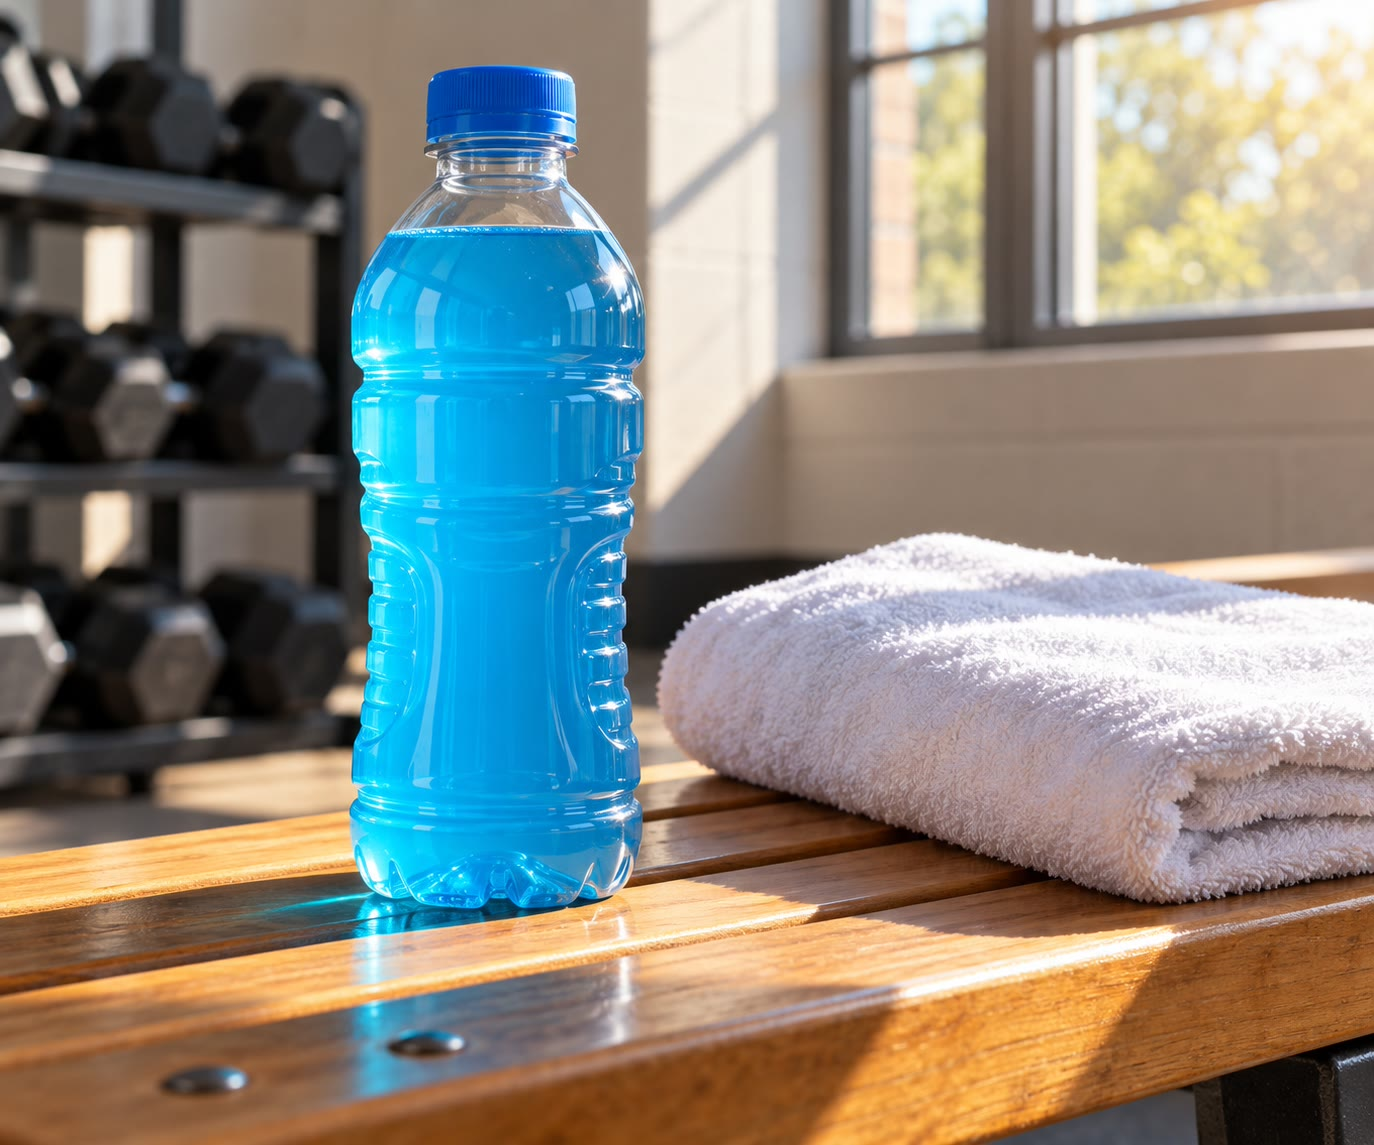
\includegraphics[width=0.5\linewidth]{images/book1/ai/g11-sports-drink.jpg}

{\small Een blauwe drank: de kleur komt van een paar milligram kleurstof
per liter.}
\end{omfigure}

\section{De kleur van een oplossing}

Wit licht, zoals daglicht, is een \omterm{def:g6:pure-substances-and-mixtures:mixture}{mengsel} van alle kleuren van de
regenboog. Elke kleur hoort bij een golflengte, van ongeveer
\qty{400}{nm} voor violet tot ongeveer \qty{750}{nm} voor rood; het
natuurkundeboek legt uit wat een golflengte is, en hier is het alleen een
etiket voor een kleur. Een gekleurde oplossing neemt een deel van het
licht op dat erdoorheen gaat, sommige kleuren veel meer dan andere; het
oog ziet de kleuren die doorgelaten worden.

\begin{definition}[Complementaire kleuren]\label{def:g11:absorbance:complementary}
Twee kleuren zijn \emph{complementaire kleuren}\index{complementaire kleuren}
als ze samen wit licht geven. Op een kleurencirkel staan complementaire
kleuren tegenover elkaar.
\end{definition}

\begin{omfigure}
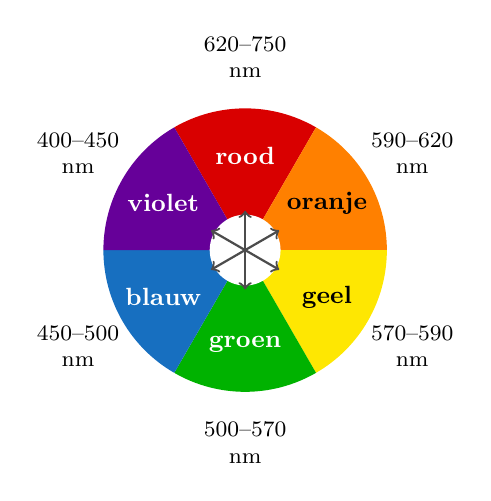
\begin{tikzpicture}[font=\small]
  \foreach \a/\c/\n/\w/\t in {90/red!85!black/rood/{620--750}/white,
      30/orange/oranje/{590--620}/black, -30/yellow!90!orange/geel/{570--590}/black,
      -90/green!70!black/groen/{500--570}/white, -150/cyan!50!blue/blauw/{450--500}/white,
      150/violet!80!blue/violet/{400--450}/white} {
    \fill[\c] (0,0) -- (\a-30:1.8) arc[start angle=\a-30, end angle=\a+30,
      radius=1.8] -- cycle;
    \node[text=\t, font=\small\bfseries] at (\a:1.2) {\n};
    \node[font=\footnotesize, align=center] at (\a:2.45) {\w\\ nm};
  }
  \fill[white] (0,0) circle (0.45);
  \draw[<->, thick, black!70] (90:0.5) -- (-90:0.5);
  \draw[<->, thick, black!70] (30:0.5) -- (-150:0.5);
  \draw[<->, thick, black!70] (-30:0.5) -- (150:0.5);
\end{tikzpicture}

{\small Een kleurencirkel, met bij benadering de golflengten.
\omterm{def:g11:absorbance:complementary}{Complementaire kleuren} staan tegenover elkaar: rood en groen, oranje en
blauw, geel en violet.}
\end{omfigure}

\begin{proposition}[De kleur die je ziet]\label{prop:g11:absorbance:colour-seen}
Een oplossing die vooral één kleur van wit licht opneemt, heeft de kleur
die daarmee complementair is.
\end{proposition}

\begin{proof}
Aangenomen: het licht dat doorgaat, is wit licht min de opgenomen kleur,
en het oog ziet die rest als de complementaire kleur.
\end{proof}

\begin{example}[Twee voedingskleurstoffen]\label{ex:g11:absorbance:dyes}
% ledger: lmax:E133, lmax:E102
De blauwe kleurstof van de sportdrank, bekend als briljantblauw (E133),
neemt vooral oranjerood licht op, rond \qty{629}{nm}: ze ziet er blauw
uit. De gele kleurstof tartrazine (E102) neemt vooral violetblauw licht
op, rond \qty{427}{nm}: ze ziet er geel uit. Een groene drank bevat meestal
allebei.
\end{example}

\section{Het absorptiespectrum}

\begin{definition}[Absorptiespectrum]\label{def:g11:absorbance:spectrum}
Het \emph{absorptiespectrum}\index{absorptiespectrum} van een oplossing is
de grafiek van het licht dat ze opneemt (haar \omterm{def:g11:absorbance:absorbance}{absorbantie}, gedefinieerd
in de volgende paragraaf) uitgezet tegen de golflengte. De golflengte
waarbij de absorptie het grootst is, schrijf je als $\lambda_{\max}$.
\end{definition}

\begin{omfigure}
\begin{tikzpicture}
\begin{axis}[width=0.85\linewidth, height=6cm, xmin=380, xmax=750,
    ymin=0, ymax=0.95, xlabel={golflengte $\lambda$ (\si{nm})},
    ylabel={absorbantie $A$}, axis lines*=left, ymajorgrids,
    grid style={gray!20}, tick label style={font=\small},
    label style={font=\small}, xtick={400,450,500,550,600,650,700,750},
    ]
  % ledger: lmax:E133, abs:E133, lmax:E102, abs:E102 (band shapes synthetic)
  \addplot[very thick, cyan!60!blue] table[x=lambda, y=E133]
    {figdata/out/grade-11-absorbance-a.dat};
  \addplot[very thick, orange!85!yellow] table[x=lambda, y=E102]
    {figdata/out/grade-11-absorbance-a.dat};
  \node[font=\small, align=left, anchor=west, text=cyan!60!blue!80!black]
    at (axis cs:668,0.62) {blauw, E133,\\ \qty{5.0}{mg/L}};
  \node[font=\small, align=left, anchor=west, text=orange!80!black]
    at (axis cs:470,0.66) {geel, E102,\\ \qty{15}{mg/L}};
  \addplot[dashed, black!50] coordinates {(629,0) (629,0.82)};
  \addplot[dashed, black!50] coordinates {(427,0) (427,0.795)};
  \node[font=\small, anchor=south] at (axis cs:629,0.83) {\qty{629}{nm}};
  \node[font=\small, anchor=south] at (axis cs:427,0.81) {\qty{427}{nm}};
\end{axis}
\end{tikzpicture}

{\small \omterm{def:g11:absorbance:spectrum}{Absorptiespectra} van de twee kleurstoffen in water, in een cuvet
van \qty{1}{cm} dik. De vorm van de banden is getekend met een eenvoudig
model; de plaats van de maxima en hun hoogte komen uit de specificaties
van de twee kleurstoffen.}
\end{omfigure}

\begin{remark}[Een spectrum lezen]\label{rem:g11:absorbance:reading}
De blauwe kleurstof neemt onder \qty{520}{nm} bijna niets op: blauw en
violet licht gaan erdoor, en de oplossing ziet er blauw uit. De gele
kleurstof neemt boven \qty{520}{nm} bijna niets op: groen, geel, oranje
en rood licht gaan erdoor, en het oog ziet geel. Bij \qty{629}{nm} neemt
alleen de blauwe kleurstof op; bij \qty{427}{nm} bijna alleen de gele.
\end{remark}

\section{Absorbantie en de spectrofotometer}

\begin{definition}[Absorbantie]\label{def:g11:absorbance:absorbance}
De \emph{absorbantie}\index{absorbantie} $A$ van een oplossing, bij een
gekozen golflengte, is het getal dat een spectrofotometer aangeeft, die
meet hoeveel licht van die golflengte de oplossing opneemt. Ze heeft geen
eenheid; ze is nul voor het zuivere \omterm{def:g6:solutions-and-solubility:solute}{oplosmiddel}, en groter naarmate de
oplossing meer licht opneemt.
\end{definition}

\begin{omfigure}
\begin{tikzpicture}[font=\small]
  % lamp
  \shade[ball color=yellow!40] (0,0.6) circle (0.32);
  \foreach \a in {0,45,90,135,180,225,270,315} \draw[yellow!60!orange, thick] (\a:0.4) ++(0,0.6) -- ++(\a:0.18);
  \node[anchor=north] at (0,-0.25) {lamp};
  \draw[black!60, thick] (0.8,0.6) -- (1.75,0.6);
  % prism
  \fill[cyan!10, draw=black!60] (1.75,0.15) -- (2.55,0.15) -- (2.15,1.15) -- cycle;
  \node[anchor=north] at (2.15,-0.25) {prisma};
  \foreach \c/\d in {violet/0.35, blue/0.22, green!70!black/0.08, yellow!90!orange/-0.06,
      orange/-0.2, red/-0.34}
    \draw[\c, thick] (2.45,0.6) -- (3.45,{0.6+\d});
  % slit
  \fill[black!70] (3.5,0.92) rectangle (3.6,1.4);
  \fill[black!70] (3.5,-0.2) rectangle (3.6,0.52);
  \node[anchor=north] at (3.55,-0.25) {spleet};
  \draw[orange, very thick] (3.6,0.6) -- (4.75,0.6);
  % cuvette
  \pic (cv) at (5,0) {cuvette={0.75}{cyan!50!blue!45}};
  \node[anchor=north] at (5,-0.25) {cuvet};
  \draw[orange!60, thick] (5.3,0.6) -- (6.3,0.6);
  % detector and display
  \fill[black!15, draw=black!60] (6.3,0.2) rectangle (6.9,1.0);
  \node[anchor=north] at (6.6,-0.25) {detector};
  \draw[black!60] (6.9,0.6) -- (7.4,0.6);
  \fill[black!80, draw=black] (7.4,0.25) rectangle (9.4,0.95);
  \node[green!70!white, font=\footnotesize\ttfamily] at (8.4,0.6) {A = 0.590};
  \node[anchor=north] at (8.4,-0.25) {display};
\end{tikzpicture}

{\small Principe van een spectrofotometer. Een prisma spreidt wit licht
in zijn kleuren uit; een spleet laat maar één golflengte door, door de
gebruiker gekozen; de detector vergelijkt het licht dat de cuvet verlaat
met het licht dat erin gaat, en het display geeft de \omterm{def:g11:absorbance:absorbance}{absorbantie}.}
\end{omfigure}

\begin{remark}[Waar het getal vandaan komt]\label{rem:g11:absorbance:log}
De \omterm{def:g11:absorbance:absorbance}{absorbantie} wordt door het instrument berekend uit de intensiteit van
het licht dat de oplossing in gaat en uit komt, met een wiskundige functie
die je in het laatste schooljaar tegenkomt, de logaritme. Een
universiteitsdeel geeft de formule; hier is de \omterm{def:g11:absorbance:absorbance}{absorbantie} gewoon wat het
instrument aanwijst.
\end{remark}

\begin{inthelab}[De spectrofotometer op nul zetten]
De cuvet, het \omterm{def:g6:solutions-and-solubility:solute}{oplosmiddel} en het instrument zelf nemen een beetje licht
op. Vóór elke meting wordt een cuvet gevuld met het zuivere \omterm{def:g6:solutions-and-solubility:solute}{oplosmiddel},
de \emph{blanco}, in het instrument gezet, en dat wordt zo ingesteld dat
het bij de gekozen golflengte $A = 0$ aangeeft. Elke meting daarna is de
\omterm{def:g11:absorbance:absorbance}{absorbantie} van de \omterm{def:g6:solutions-and-solubility:solute}{opgeloste stof} alleen. Cuvetten pak je altijd vast aan
hun matte zijden, en je veegt ze af: een vingerafdruk op een heldere
zijde neemt ook licht op.
\end{inthelab}

\begin{omfigure}
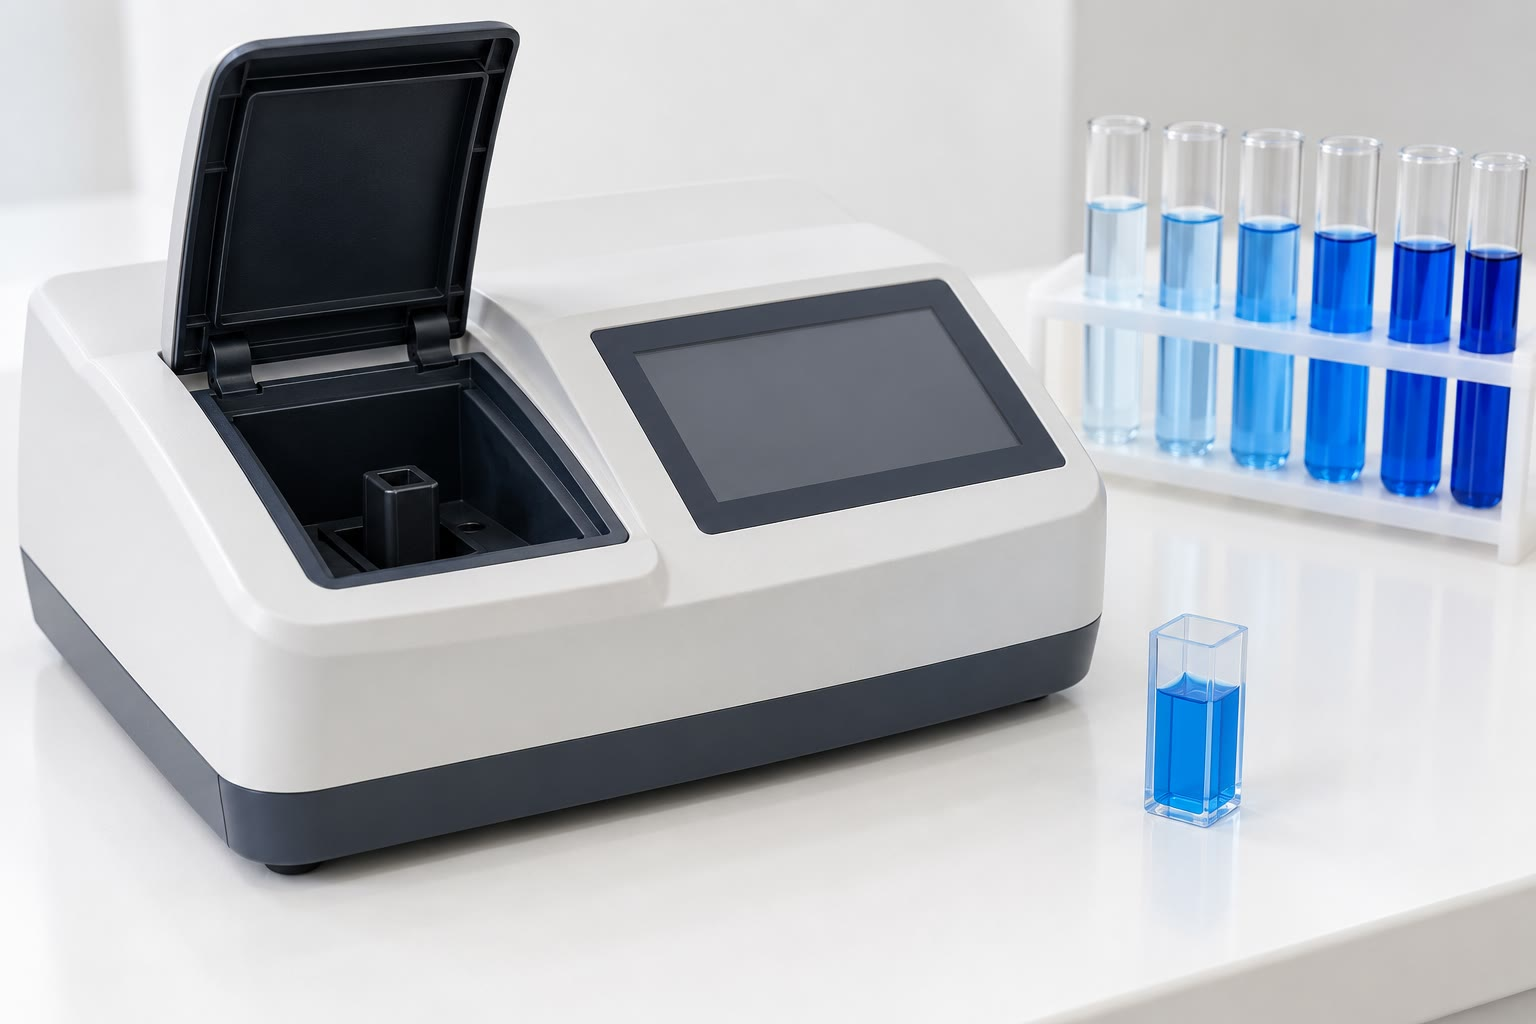
\includegraphics[width=0.5\linewidth]{images/book1/ai/g11-spectrophotometer.jpg}

{\small Een spectrofotometer met zijn vierkante cuvetten.}
\end{omfigure}

\section{De wet van Lambert-Beer}

\begin{definition}[Molaire absorptiecoëfficiënt]\label{def:g11:absorbance:epsilon}
De \emph{molaire absorptiecoëfficiënt}\index{molaire absorptiecoëfficiënt}
$\varepsilon$ van een \omterm{def:g6:solutions-and-solubility:solute}{opgeloste stof}, bij een gegeven golflengte, geeft
aan hoe sterk één \omterm{def:g10:the-mole:amount}{mol} ervan licht opneemt; hij hangt af van de stof, het
\omterm{def:g6:solutions-and-solubility:solute}{oplosmiddel} en de golflengte, en wordt uitgedrukt in \si{L/(mol.cm)}.
\end{definition}

\begin{proposition}[Wet van Lambert-Beer]\label{prop:g11:absorbance:beer-lambert}
Voor een verdunde oplossing van één enkele absorberende stof, met \omterm{def:g10:concentration-and-dilution:molar-concentration}{molaire
concentratie} $c$, in een cuvet met dikte $\ell$, is de \omterm{def:g11:absorbance:absorbance}{absorbantie} bij
een gegeven golflengte
\[
  A = \varepsilon\, \ell\, c .
\]
De \omterm{def:g11:absorbance:absorbance}{absorbantie} is evenredig met de concentratie.
\end{proposition}

\begin{proof}
Hier aangenomen; ze wordt afgeleid in een universiteitsdeel.
\end{proof}


\begin{remark}[Met een massaconcentratie]\label{rem:g11:absorbance:mass}
% ledger: abs:E133, mw:E133
Omdat $c = C_m / M$, kun je de wet ook schrijven als $A = a\, \ell\, C_m$,
met $a = \varepsilon / M$ in \si{L/(g.cm)}. De specificaties van
voedingskleurstoffen geven $a$: voor de blauwe kleurstof E133 bij
\qty{629}{nm} is $a =
\qty{164}{L/(g.cm)}$, en met haar \omterm{def:g10:the-mole:molar-mass}{molaire massa} van \qty{792.9}{g/mol} is
$\varepsilon = 164 \times 792.9 = \qty{1.30e5}{L/(mol.cm)}$. Een oplossing
van maar \qty{5.0}{mg/L} ervan geeft in een cuvet van \qty{1}{cm} al
$A = 164 \times 1 \times 0.0050 = 0.82$.
\end{remark}

\begin{remark}[Alleen verdunde oplossingen]\label{rem:g11:absorbance:dilute}
De evenredigheid geldt alleen voor verdunde oplossingen, in de praktijk
voor \omterm{def:g11:absorbance:absorbance}{absorbanties} onder ongeveer 1 tot 1.5 op een gewoon instrument. Een
oplossing die te geconcentreerd is, wordt eerst met een bekende factor
verdund en dan gemeten.
\end{remark}

\section{Een concentratie meten}

\begin{definition}[IJklijn]\label{def:g11:absorbance:calibration-line}
Een \emph{ijklijn}\index{ijklijn} is de grafiek van de \omterm{def:g11:absorbance:absorbance}{absorbantie} van een
reeks \omterm{def:g10:concentration-and-dilution:standard}{standaardoplossingen} van één stof, gemeten bij dezelfde golflengte
in dezelfde cuvet, uitgezet tegen hun concentratie. Als de wet van
Lambert-Beer geldt, is het een rechte lijn door de oorsprong.
\end{definition}

\begin{method}[Een concentratie meten met een ijklijn]\label{met:g11:absorbance:calibration}
\begin{enumerate}
  \item Neem het \omterm{def:g11:absorbance:spectrum}{absorptiespectrum} van de stof op en kies de golflengte
        $\lambda_{\max}$, waar de \omterm{def:g11:absorbance:absorbance}{absorbantie} het grootst is en het minst
        verandert bij een kleine fout in de golflengte.
  \item Zet het instrument op nul met de blanco.
  \item Maak \omterm{def:g10:concentration-and-dilution:standard}{standaardoplossingen} door een \omterm{def:g10:concentration-and-dilution:dilution}{stamoplossing} te verdunnen en
        meet hun \omterm{def:g11:absorbance:absorbance}{absorbanties}.
  \item Zet $A$ uit tegen de concentratie en trek de rechte lijn door de
        oorsprong die het best bij de punten past.
  \item Meet de onbekende, zo nodig verdund zodat haar \omterm{def:g11:absorbance:absorbance}{absorbantie} tussen
        die van de standaarden ligt, en lees haar concentratie af op de
        lijn (of deel $A$ door de richtingscoëfficiënt); vermenigvuldig
        met de \omterm{def:g10:concentration-and-dilution:dilution}{verdunningsfactor}.
\end{enumerate}
\end{method}

\begin{omfigure}
\begin{tikzpicture}
\begin{axis}[width=0.72\linewidth, height=6cm, xmin=0, xmax=5.6,
    ymin=0, ymax=0.95, xlabel={concentratie E133 (\si{mg/L})},
    ylabel={absorbantie bij \qty{629}{nm}}, axis lines*=left, ymajorgrids,
    xmajorgrids, grid style={gray!20}, tick label style={font=\small},
    label style={font=\small}]
  % ledger: abs:E133 (points synthetic: exact values + fixed offsets)
  \addplot[only marks, mark=*, mark size=2.2pt, omDef] table[x=C, y=A]
    {figdata/out/grade-11-absorbance-b.dat};
  \addplot[thick, omProp, domain=0:5.5] {0.164*x};
  \addplot[dashed, black!60] coordinates {(0,0.590) (3.6,0.590) (3.6,0)};
  \node[font=\small, anchor=south west] at (axis cs:0.1,0.6) {onbekend: $A = 0.590$};
  \node[font=\small, anchor=west] at (axis cs:3.65,0.22) {\qty{3.6}{mg/L}};
\end{axis}
\end{tikzpicture}

{\small IJklijn van de blauwe kleurstof: vijf standaarden (punten) en de
lijn door de oorsprong, met richtingscoëfficiënt \qty{0.164}{L/mg}. Een
onbekende met $A = 0.590$ heeft een concentratie van $0.590 / 0.164 =
\qty{3.6}{mg/L}$.}
\end{omfigure}

\begin{example}[De vijf standaarden]\label{ex:g11:absorbance:standards}
Een \omterm{def:g10:concentration-and-dilution:dilution}{stamoplossing} van de blauwe kleurstof met \qty{100}{mg/L} wordt
verdund tot \qty{100.0}{mL} van elke standaard: voor \qty{2.0}{mg/L} is
de \omterm{def:g10:concentration-and-dilution:dilution}{verdunningsfactor} 50, dus wordt \qty{2.0}{mL} \omterm{def:g10:concentration-and-dilution:dilution}{stamoplossing} aangevuld
tot \qty{100.0}{mL}. De vijf standaarden, van 1 tot \qty{5}{mg/L}, geven
0.168, 0.325, 0.494, 0.652 en 0.823: op een paar duizendsten na gelijk
aan $0.164 \times C$, de lijn van de figuur.
\end{example}

\section{Oefeningen}

\begin{exercise}[$\star$]\label{exo:g11:absorbance:1}
Een oplossing neemt vooral oranje licht op. Welke kleur heeft ze? En een
oplossing die vooral violet licht opneemt?
\end{exercise}

\begin{exercise}[$\star$]\label{exo:g11:absorbance:2}
Geef met de kleurencirkel de kleur die een groene oplossing vooral
opneemt, en het gebied van golflengten dat bij die kleur hoort.
\end{exercise}

\begin{exercise}[$\star$]\label{exo:g11:absorbance:3}
Lees op de \omterm{def:g11:absorbance:spectrum}{absorptiespectra} de golflengte $\lambda_{\max}$ van elke
kleurstof af, en de \omterm{def:g11:absorbance:absorbance}{absorbantie} daar.
\end{exercise}

\begin{exercise}[$\star$]\label{exo:g11:absorbance:4}
Een kleurstofoplossing met \qty{2.0}{mg/L} geeft $A = 0.30$. Wat geeft een
oplossing van dezelfde kleurstof met \qty{6.0}{mg/L} in dezelfde cuvet,
bij dezelfde golflengte? En met \qty{1.0}{mg/L}?
\end{exercise}

\begin{exercise}[$\star$]\label{exo:g11:absorbance:5}
Wat is de blanco van een spectrofotometer, en waarom zet je het
instrument ermee op nul?
\end{exercise}

\begin{exercise}[$\star\star$]\label{exo:g11:absorbance:6}
Bepaal met de \omterm{def:g11:absorbance:calibration-line}{ijklijn} van de blauwe kleurstof de concentratie van een
oplossing die $A = 0.41$ geeft.
\end{exercise}

\begin{exercise}[$\star\star$]\label{exo:g11:absorbance:7}
Waarom zet je de spectrofotometer voor de blauwe kleurstof op
\qty{629}{nm} en niet op \qty{550}{nm}? Geef twee redenen.
\end{exercise}

\begin{exercise}[$\star\star$]\label{exo:g11:absorbance:8}
Een onverdunde drank geeft $A = 2.4$ bij \qty{629}{nm}, te hoog om te
vertrouwen. Hij wordt vijf keer verdund en geeft dan $A = 0.48$. Bepaal
de concentratie blauwe kleurstof in de drank.
\end{exercise}

\begin{exercise}[$\star\star$]\label{exo:g11:absorbance:9}
% ledger: mw:E102, abs:E102
Een oplossing van tartrazine met \qty{15.0}{mg/L} geeft $A = 0.795$ bij
\qty{427}{nm} in een cuvet van \qty{1.00}{cm}. Bereken haar
absorptiviteit $a$ in \si{L/(g.cm)}, en daarna haar \omterm{def:g11:absorbance:epsilon}{molaire
absorptiecoëfficiënt} (\omterm{def:g10:the-mole:molar-mass}{molaire massa} \qty{534.4}{g/mol}).
\end{exercise}

\begin{exercise}[$\star\star$]\label{exo:g11:absorbance:10}
Kijk naar de spectra van de twee kleurstoffen. Boven welke golflengte
neemt de gele kleurstof bijna niets op? Waarom kun je de blauwe kleurstof
bij \qty{629}{nm} meten, zelfs in een groene drank die ook de gele
kleurstof bevat?
\end{exercise}

\begin{exercise}[$\star\star$]\label{exo:g11:absorbance:11}
Dezelfde oplossing wordt gemeten in een cuvet van \qty{2.0}{cm} dik in
plaats van \qty{1.0}{cm}. Hoe verandert de \omterm{def:g11:absorbance:absorbance}{absorbantie}? Waarom?
\end{exercise}

\begin{exercise}[$\star\star\star$]\label{exo:g11:absorbance:12}
Standaarden van de blauwe kleurstof met 5, 10, 20 en \qty{40}{mg/L} geven
0.82, 1.62, 2.30 en 2.70. Bereken voor elke standaard $A / C$. Wat valt je
op? Welke standaarden mag je voor een \omterm{def:g11:absorbance:calibration-line}{ijklijn} gebruiken, en wat moet er
gebeuren met een onbekende die $2.5$ geeft?
\end{exercise}

\begin{exercise}[$\star\star\star$]\label{exo:g11:absorbance:13}
Een groene drank bevat de blauwe en de gele kleurstof. In een cuvet van
\qty{1.00}{cm} geeft hij $A = 0.574$ bij \qty{629}{nm} en $A = 0.53$
bij \qty{427}{nm}. Bij \qty{427}{nm} neemt de blauwe kleurstof bijna niets
op, en bij \qty{629}{nm} neemt de gele kleurstof niets op. Bepaal de
\omterm{def:g10:concentration-and-dilution:mass-concentration}{massaconcentraties} van beide kleurstoffen (gebruik
$a = \qty{164}{L/(g.cm)}$ en $a = \qty{53.0}{L/(g.cm)}$).
\end{exercise}

\begin{exercise}[$\star\star\star$]\label{exo:g11:absorbance:14}
Een leerling vergeet de blanco en zet het instrument op nul met een lege
cuvet. Elke meting is dan \num{0.040} te hoog. De onbekende geeft
$0.368$, en ze deelt door de richtingscoëfficiënt $0.164$ van de echte
\omterm{def:g11:absorbance:calibration-line}{ijklijn}. Welke concentratie vindt ze? Wat is de echte? Met welk
percentage zit ze ernaast?
\end{exercise}

\begin{exercise}[$\star\star\star$]\label{exo:g11:absorbance:15}
% ledger: adi:E102
De aanvaardbare dagelijkse inname van tartrazine is \qty{10}{mg} per
kilogram lichaamsmassa. Een drank bevat er \qty{20}{mg/L} van. Welk volume
van de drank zou een volwassene van \qty{60}{kg} op één dag tot deze
inname brengen? Is dat een realistisch risico?
\end{exercise}

\section{Probleem: Het blauw van een sportdrank}


\begin{problem}[{Weekendprobleem --- hoeveel flessen blauwe sportdrank zou
een kind moeten drinken om de veilige daggrens van de kleurstof te
bereiken?}]
\label{pb:g11:absorbance:1}
% ledger: lmax:E133, abs:E133, mw:E133, adi:E133
Een voedingslaboratorium controleert de blauwe kleurstof E133 van een
sportdrank die in flessen van \qty{500}{mL} verkocht wordt. De
specificaties van de kleurstof geven haar \omterm{def:g10:the-mole:molar-mass}{molaire massa},
\qty{792.9}{g/mol}, en haar aanvaardbare dagelijkse inname: \qty{6}{mg}
per kilogram lichaamsmassa per dag, een hoeveelheid die je een leven lang
elke dag kunt binnenkrijgen zonder noemenswaardig risico.

\medskip
\noindent\textbf{Deel I --- Kleur en spectrum.}
\begin{enumerate}
  \item De drank ziet er blauw uit. Welke kleur licht neemt hij volgens de
        kleurencirkel het meest op?
  \item Lees de golflengte $\lambda_{\max}$ van de kleurstof af op haar
        spectrum.
  \item Waarom is de \omterm{def:g11:absorbance:absorbance}{absorbantie} van de kleurstof bij \qty{450}{nm} bijna
        nul? Past dat bij haar kleur?
  \item Bij welke golflengte moeten de metingen gedaan worden?
\end{enumerate}

\medskip
\noindent\textbf{Deel II --- De \omterm{def:g11:absorbance:calibration-line}{ijklijn}.}
\begin{enumerate}[resume]
  \item Er wordt \qty{50.0}{mg} zuivere kleurstof opgelost tot
        \qty{500.0}{mL} \omterm{def:g10:concentration-and-dilution:dilution}{stamoplossing}. Bereken de \omterm{def:g10:concentration-and-dilution:mass-concentration}{massaconcentratie} in
        \si{mg/L}.
  \item Er worden standaarden van 1.0, 2.0, 3.0, 4.0 en \qty{5.0}{mg/L}
        gemaakt, elk \qty{100.0}{mL}. Hoeveel \omterm{def:g10:concentration-and-dilution:dilution}{stamoplossing} is er nodig
        voor de standaard van \qty{3.0}{mg/L}? Met welk glaswerk?
  \item De standaarden geven 0.168, 0.325, 0.494, 0.652 en 0.823. Bereken
        voor elke standaard $A / C$, en laat zien dat de punten dicht bij
        een lijn door de oorsprong liggen met een richtingscoëfficiënt van
        ongeveer \qty{0.164}{L/mg}.
  \item Waarom moet de lijn door de oorsprong gaan?
  \item Leid daaruit de absorptiviteit $a$ van de kleurstof af in
        \si{L/(g.cm)} (cuvet van \qty{1.00}{cm}), en daarna haar \omterm{def:g11:absorbance:epsilon}{molaire
        absorptiecoëfficiënt}.
\end{enumerate}

\medskip
\noindent\textbf{Deel III --- De drank.}
\begin{enumerate}[resume]
  \item Er wordt \qty{25.0}{mL} drank met water aangevuld tot
        \qty{50.0}{mL}. Wat is de \omterm{def:g10:concentration-and-dilution:dilution}{verdunningsfactor}?
  \item De verdunde drank geeft $A = 0.590$. Bepaal de concentratie
        kleurstof.
  \item Leid daaruit de concentratie kleurstof in de drank zelf af.
  \item Wat zou de onverdunde drank aangeven? Waarom werd hij verdund?
  \item Bereken de massa kleurstof in één fles.
  \item Bereken de hoeveelheid kleurstof, in \omterm{def:g10:the-mole:amount}{mol}, in één fles.
\end{enumerate}

\medskip
\noindent\textbf{Deel IV --- De aanvaardbare dagelijkse inname.}
\begin{enumerate}[resume]
  \item Hoeveel van de kleurstof mag een kind van \qty{30}{kg} per dag
        binnenkrijgen?
  \item Hoeveel flessen zou het kind op één dag moeten drinken om die
        grens te bereiken?
  \item Welk volume drank is dat? Geef commentaar.
  \item Dezelfde vraag voor een volwassene van \qty{70}{kg}.
  \item Geef het eindantwoord: hoeveel flessen van \qty{500}{mL} zou een
        kind van \qty{30}{kg} op één dag moeten drinken om de
        aanvaardbare dagelijkse inname van de kleurstof te bereiken?
\end{enumerate}
\end{problem}
